\documentclass[a4paper,12pt]{article} % тип документа
\usepackage[margin=1in]{geometry} % Поля

%  Русский язык
\usepackage[warn]{mathtext}
\usepackage[T2A]{fontenc}			% кодировка
\usepackage[utf8]{inputenc}			% кодировка исходного текста
\usepackage[english,russian]{babel}	% локализация и переносы
% Математика
\usepackage{amsmath,amsfonts,amssymb,amsthm,mathtools} 
\usepackage{wasysym}
%%%
\usepackage{graphicx}

\usepackage{tabularx}

\usepackage{gensymb} % знак градуса
\usepackage{enumitem} % изменить список enumerate
\usepackage{placeins} % \FloatBarrier

\renewcommand{\thesection}{\Roman{section}} 
\renewcommand{\thesubsection}{\roman{subsection}}


\begin{document}

\newcolumntype{Y}{>{\centering\arraybackslash}X} %new tabularx


%титул
\hrule 	
\medskip
\begin{raggedright}
{\large \textbf{Отчёт по работе №23}}
\\
\medskip
{\Large Изучение электропроводности и определение удельного сопротивления полупроводников} 
\\
\medskip
{\large Карташов Констанин Б04-005}
\medskip
\hrule
\medskip
\end{raggedright}



\section{Экспериментальная часть}

\subsection{Установка}

\begin{figure}[h]
\centering
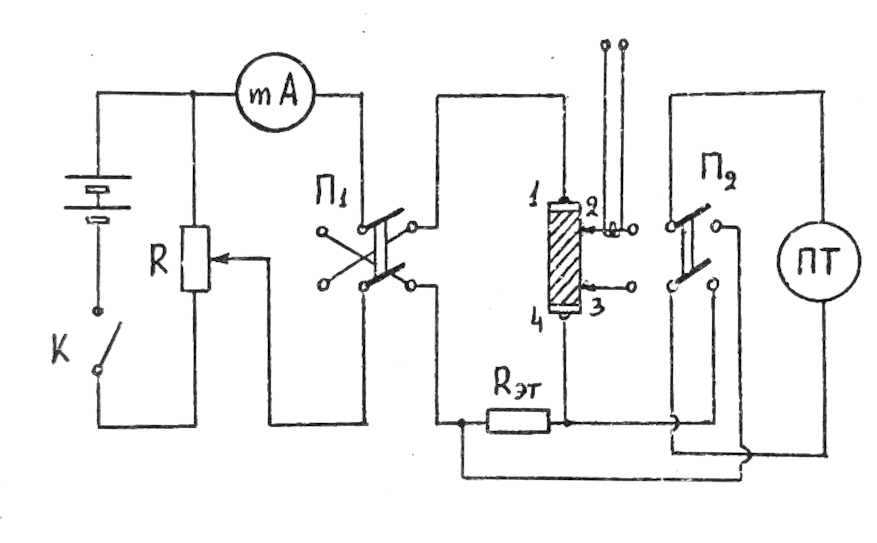
\includegraphics[width=0.5\textwidth]{setup.png}
\caption{Принципиальная схема двухзоднового метода измерения удельного сопротивления полупроводникового образца.}
\label{fig:setup}
\end{figure}

\paragraph{} В данной работе для измерения удельного сопротивления используется двухзодновый метод, так как у нас образец правильной геометрической формы (цилиндр). Принципиальная схема метода приведена на рис. \ref{fig:setup}.

На торцевые части полупроводникового образца наносятся токовые металлические контакты и образец зажимают между двумя токопроводящими электродами (1, 4). К шлифованной боковой поверхности образца прижимают два зонда (2, 3) на расстоянии $L$ один от другого. 

В данной работе напряжение между двумя зондами измеряется компенсационным методом, ток через цепь измеряется амперметром.

\subsection{Измерения}

\begin{table}[h]
\centering
\begin{tabular}{|l|c|c|c|c|c|c|c|c|c|c|c|}
\hline
№ изм. & 1    & 2    & 3    & 4    & 5    & 6    & 7   & 8   & 9   & 10  & 11  \\ \hline
U, мВ  & 12.3 & 12.0 & 11.8 & 11.7 & 11.5 & 11.1 & 9.9 & 9.7 & 9.1 & 8.7 & 8.7 \\ \hline
№ изм. & 12   & 13   & 14   & 15   & 16   & 17   & 18  & 19  & 20  & 21  & 22  \\ \hline
U, мВ  & 7.8  & 7.4  & 7.4  & 7.1  & 6.5  & 6.6  & 5.6 & 6.0 & 5.2 & 2.9 & 3.5 \\ \hline
\end{tabular}
\caption{Таблица измеренных данных}
\label{tab:data}
\end{table}

\paragraph{} Измерения будем проводить при постоянном токе $I = 100$ мА. Посте каждого измерения будем сближать зонды на 0.5 мм, $\Delta L = -0.5$ мм, значит полное изменение расстояния между зондами будет равно $\Delta l = (n - 1) \Delta L$, где $n$ -- номер измерения, измеренные данные приведены в табл. \ref{tab:data}. Таким образом найдём зависимость $U_x = U_x(\Delta l)$. Теоретическая завимисость должна иметь вид:

\begin{equation}
U_x = I R_x = I \left( R_0 + \frac{\rho}{S} \Delta l \right) = U_0 + 4 \frac{I \rho}{\pi d^2} \Delta l,
\label{e:ux}
\end{equation}

\noindent где $\rho$ -- удельное сопротивление образца, $S$ -- площадь сечения, $d$ -- диаметр.

\subsection{Нахождение удельного сопротивления}

\begin{figure}
\centering
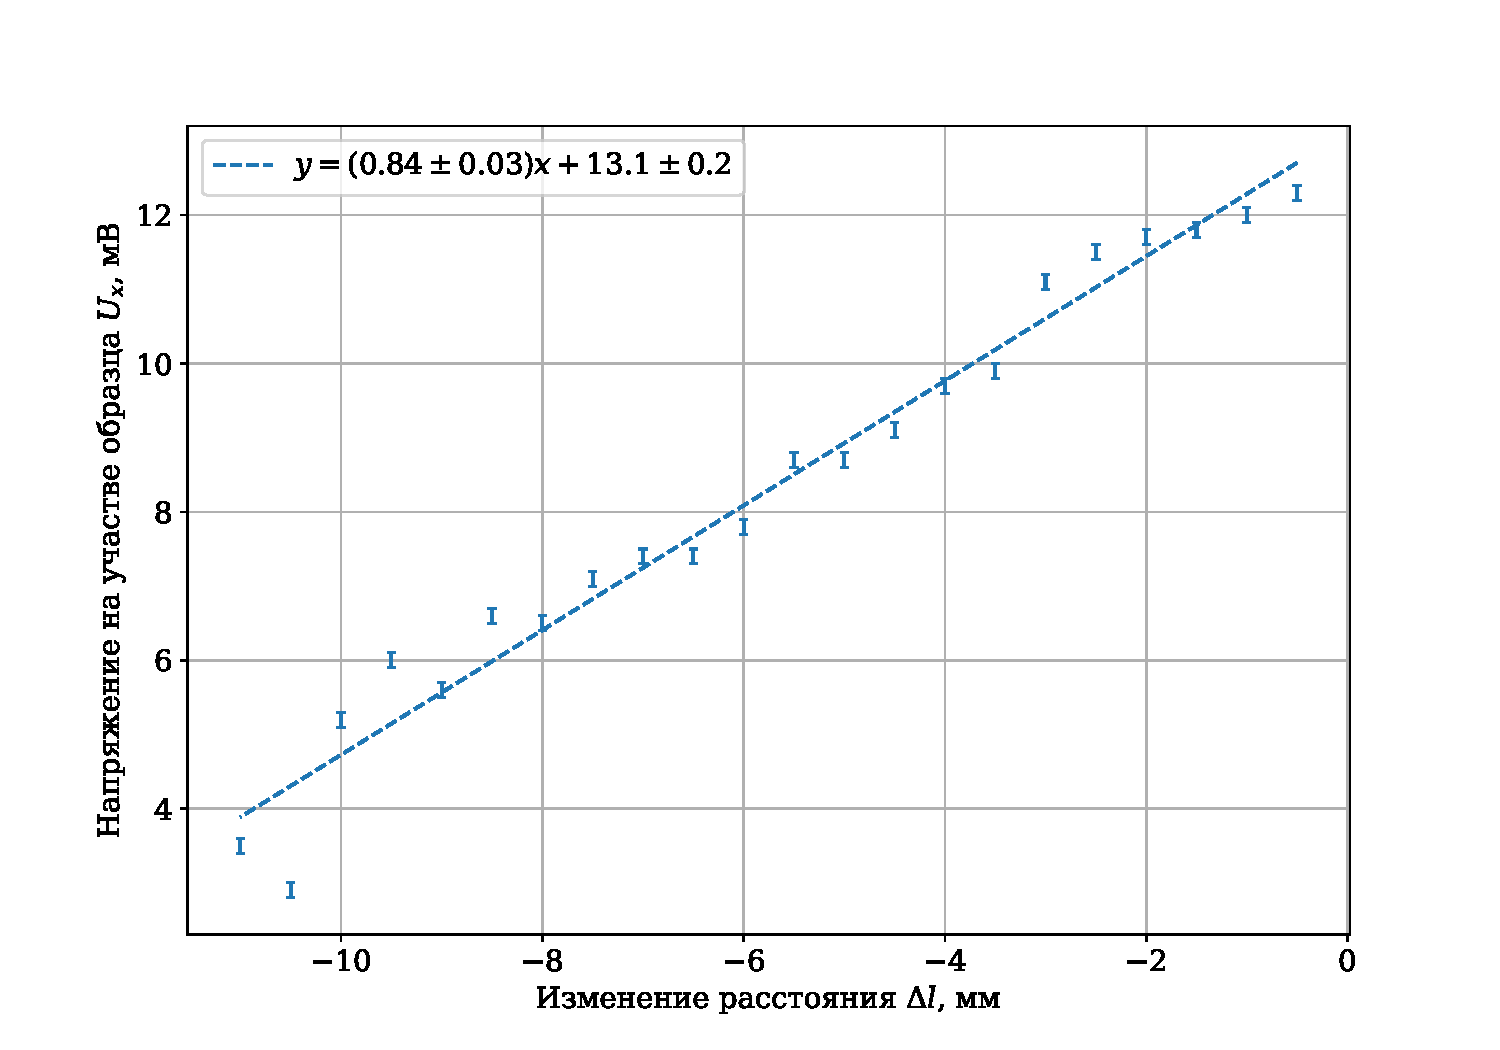
\includegraphics[width=\textwidth]{plot.pdf}
\caption{График зависимости $U_x(\Delta l)$ с проведённой наилучшей прямой.}
\label{fig:plot}
\end{figure}

\paragraph{} Построим график полученной зависимости $U_x(\Delta l)$. Основываясь на зависимости \eqref{e:ux}, построим на графике наилучшую прямую $y = ax + b$ по МНК. Полученное значение $a = 0.84 \pm 0.03$ В/м. Найдём удельное сопротивление:

\begin{equation}
4 \frac{I \rho}{\pi d^2} = a \;\;\; \Rightarrow \;\;\; \rho = \frac{\pi a d^2}{4I} = \frac{\pi \cdot (0.84 \pm 0.03) \text{В/м} \cdot (6 \text{мм})^2}{4 \cdot 100 \text{мА}} = (2.4 \pm 0.1) \cdot 10^{-4} \text{Ом} \cdot  \text{м}.
\label{e:rho}
\end{equation}



\medskip\hrule\medskip

\section{Выводы}

\begin{enumerate}
\item Получили зависимость напряжения от расстояния между зондами. Полученное соотношение хорошо ложится на прямую, что соответствен теории. При этом существуют небольшие неровности, которые могут объяснятся неровностями на поверхности образца.
\item Получили удельное сопротивление образца $\rho = (2.4 \pm 0.1) \cdot 10^{-4} \text{Ом} \cdot  \text{м}$. Это удельное сопротивление лежит в пределах сопротивлений полупроводников.
\end{enumerate}

\medskip\hrule\medskip

\end{document}
